\documentclass[conference]{IEEEtran}
\IEEEoverridecommandlockouts

\usepackage{lettrine}

\usepackage[pdfpagelabels]{hyperref}
\usepackage{url}
\usepackage{graphicx}
\usepackage{float}

\usepackage[sorting=none]{biblatex}
\addbibresource{SDCC.bib}

\begin{document}

\title{LPN: Log Partition Network}

\author{
\IEEEauthorblockN{Daniele Ferrarelli\IEEEauthorrefmark{1},
Marco Ferri\IEEEauthorrefmark{2},
Lorenzo Valeriani\IEEEauthorrefmark{3}}
\IEEEauthorblockA{\textit{Dipartimento di Ingegneria Civile e Ingegneria
Informatica}\\
\textit{Università degli studi di Roma ``Tor Vergata''}\\
Roma, Italia\\
\IEEEauthorrefmark{1}daniele.ferrarelli@alumni.uniroma2.eu\\
\IEEEauthorrefmark{2}marco.ferri.98@alumni.uniroma2.eu\\
\IEEEauthorrefmark{3}lorenzo.valeriani.459326@alumni.uniroma2.eu}
}

\pdfinfo{
  /Title    (LPN: Log Partition Network)
  /Author   (Daniele Ferrarelli, Marco Ferri, Lorenzo Valeriani)
  /Creator  (Daniele Ferrarelli, Marco Ferri, Lorenzo Valeriani)
  /Producer (Daniele Ferrarelli, Marco Ferri, Lorenzo Valeriani)
  /Subject  (LPN)
  /Keywords (LPN)
}

\maketitle

\begin{abstract}
In questo documento si illustra una soluzione implementativa di uno storage chiave-valore distribuito per edge computing scritta in Go.
\end{abstract}

\begin{IEEEkeywords}
sistemi distribuiti, peer-to-peer, edge computing, cloud computing, distributed systems, key-value storage
\end{IEEEkeywords}

\section{Introduzione}
\lettrine{\textbf{L}}{\textbf{e}} reti peer-to-peer rappresentano una soluzione comune per il problema dello storage distribuito.
Tra queste, quelle strutturate si prestano particolarmente alle tipologie di storage chiave-valore.
Attraverso tecniche come il consistent hashing, si supportano le operazioni di ricerca delle informazioni in modo efficiente.\cite{p2pLookup}
L'edge computing è un paradigma di computazione che estende il cloud tradizionale con le funzionalità di computazione e
storage offerte da nodi localizzati ai bordi della rete e quindi vicino agli utenti. La soluzione proposta sfrutta una
rete peer-to-peer strutturata per indicizzare le risorse distribuite sui vari nodi edge, cercando di trarre beneficio da entrambe le realtà.
Il protocollo utilizzato dalla rete peer-to-peer è Kademlia,\cite{kademlia} nell'implementazione in Go fornita da IPFS\cite{kadDHT}.
I dati sono replicati su più nodi affinché il sistema sia tollerante ai guasti.
La consistenza tra le repliche dei dati è affidata all'algoritmo di consenso distribuito Raft.\cite{raft}\cite{raftGolang}
Il progetto fa largo uso dei servizi cloud forniti da Amazon Web Services, quali RDS, Lambda e DynamoDB.
La comunicazione tra i nodi e con i client è attuata tramite chiamate gRPC.

\section{Topologia}
I nodi del sistema sono connessi per formare una rete peer-to-peer strutturata, su questa è presente un'ulteriore serie di collegamenti
che costituisce la rete di replicazione dei dati. Quando si inserisce un nuovo dato nel sistema, questo sarà memorizzato
almeno nel nodo che ha ricevuto l'operazione di inserimento, per far sì che la latenza di rete tra l'utente ed il dato sia minima.
Quest'ultimo nodo sarà il responsabile di quel dato, identificato da una chiave. Oltre a questo, il dato sarà replicato
su un insieme di nodi che possono essere contattati in caso di fallimento del responsabile.
I vari nodi vengono identificati tramite il loro indirizzo IP.

\subsection{Rete di indexing}
Il sistema sfrutta la DHT di Kademlia per associare ad ogni chiave memorizzata l'indirizzo IP del nodo responsabile.
Così facendo si mantiene l'efficienza del lookup di una rete strutturata (O(log(N))), permettendo di posizionare
il dato in un nodo che minimizzi la latenza con il client che vi accede. La rete peer-to-peer memorizza inoltre per ogni
nodo il cluster di replicazione a cui appartiene, in caso di crash del nodo responsabile è necessario eseguire un'altra richiesta sulla
DHT per cercare una replica attiva del dato. La complessità totale dell'operazione resta O(log(N)).
Al fine di supportare questo comportamento, si è realizzata una struttura per incapsulare la libreria fornita da IPFS,
estendendo il suo comportamento in modo trasparente alle richieste.\\
Le operazioni aggiunte sono:
\begin{itemize}
  \item {PutValue e GetValue}
  \item {PutCluster e GetCluster}
\end{itemize}
La distinzione tra le operazioni di ricerca chiave-responsabile e responsabile-cluster è eseguita impostando correttamente
il primo byte della chiave.
Allo stesso modo, in caso di ricerca chiave-responsabile, osservando il primo byte del campo corrispondente al responsabile,
è possibile capire se la chiave è presente sulla DHT oppure ha subito offloading sul cloud. I dettagli di quest'ultima
operazione sono affrontati nella corrispondente sezione.

\subsection{Rete di replicazione}
L'insieme dei nodi del sistema è partizionato in un insieme di cluster di replicazione. I nodi che appartengono allo
stesso cluster si replicano vicendevolmente e i dati sono mantenuti consistenti tramite Raft. La formazione dei cluster
avviene quando i nodi richiedono l'ingresso nel sistema. Nel caso in cui non ci siano cluster già formati, i nodi aspettano
l'ingresso di altri, per essere certi di poter assicurare un determinato livello di tolleranza ai guasti, che può essere
configurato dall'amministratore. Quando la quantità di nodi è sufficiente, questi formano un primo cluster. Gli ingressi successivi
andranno a far parte di questo cluster, finché la dimensione di quest'ultimo non sarà due volte la dimensione minima di un
cluster: in questo caso, metà dei nodi si staccheranno per formarne uno nuovo.

\section{Storage locale}
Lo storage locale di ogni nodo è stato implementato come un'interfaccia in grado di esporre le operazioni:
\begin{itemize}
  \item {\small{\verb!Get(key []byte) ([][]byte, error)!}}
  \item {\small{\verb!Put(key []byte, value [][]byte) error!}}
  \item {\small{\verb!Append(key []byte, value [][]byte)!\\ \verb!    ([][]byte, error)!}}
  \item {\small{\verb!Del(key []byte) error!}}
  \item {\small{\verb!DeleteExcept([]string) error!}}
  \item {\small{\verb!GetAllKeys() ([]string, []string)!}}
\end{itemize}
L'uso di un'interfaccia permette un'astrazione a livello di codice ed una migliore semplicità di espansione del progetto
al fine di supportare diverse tecnologie di storage. Attualmente, sono fornite due implementazioni della stessa interfaccia:
una che fa uso di BadgerDB, on-disk, e l'altra di Redis, in-memory. L'interfaccia che sfrutta Redis, in particolare, si collega ad un indirizzo
IP, che può essere esposto da un container. Alcune operazioni, come l'append, richiedono un'esecuzione transazionale dal
momento che sfruttano una get seguita da una put. In Redis, sono state sfruttate le condizioni di lock ottimistico secondo
le quali una transazione è mandata in abort e fatta ripartire in caso di race condition nei confronti della stessa chiave.

\section{Consistenza e tolleranza ai guasti}
Al fine di garantire tolleranza ai guasti, tutti i dati sono replicati all'interno di un cluster. Le varie repliche sono tenute aggiornate
tramite Raft. L'algoritmo, prevedendo la presenza di un leader, garantisce l'ordinamento sequenziale delle operazioni
secondo il suo ordine di programma. Si è tuttavia scelto di gestire le operazioni di get esternamente a Raft: nel caso
in cui il dato sia presente sulla replica contattata, quest'ultima lo ritorna immediatamente, anche se potrebbe non essere
la versione più aggiornata. Gli errori supportati sono solamente errori temporanei: se un nodo subisce crash, si assume
che questo tornerà ad essere disponibile dopo un intervallo finito di tempo. La quantità massima di crash gestibili
in un singolo cluster in contemporanea dipende dalla dimensione minima del cluster configurata: per gestire k errori la
dimensione deve essere \(2k+1\). È opportuno notare che, essendo la dimensione di un cluster compresa tra \(2k+1\) e
\(4k+1\), i cluster più grandi potrebbero essere in grado di tollerare più di k guasti. I nodi comunicano tra loro e con
i client tramite chiamate gRPC. La semantica di errore nelle chiamate a procedura remota è stata resa at-least-once impostando
una policy di retry nella configurazione di gRPC.

\section{Migrazione}
Il sistema supporta la migrazione delle chiavi da un nodo ad un altro. Questa operazione viene richiesta automaticamente
in base alla quantità di operazioni richiese dai client ad un nodo nei confronti di una singola chiave. È possibile configurare
un peso per le operazioni di scrittura, ovvero put e append, e per le operazioni di lettura, ovvero get. Si mantengono
in memoria per ogni nodo le operazioni richieste recentemente dai client e verso quali chiavi.
Si può configurare per quanto tempo tenere traccia delle operazioni ricevute. Tutte le operazioni ricevute e le chiavi
alle quali queste si riferiscono sono memorizzate in una struttura dati ordinata nel tempo, supportata da una slice.
Quando si accede a questa struttura, si tiene conto del tempo attuale e si eliminano tutte le operazioni ritenute obsolete.
La ricerca dell'indice dell'ultima operazione da rimuovere, essendo la struttura dati ordinata, avviene tramite ricerca
binaria. Una volta trovata questa si rimuovono tutte le operazioni precedenti. Una singola goroutine gestisce l'accesso a questa
struttura per evitare la necessità di sincronizzazione e, allo scadere di un intervallo configurabile, la scorre interamente,
valutando per ogni chiave la quantità di operazioni che la riguardano ed il costo di queste. Nel caso in cui la somma dei
costi per ogni operazione di una chiave superi una soglia configurabile, il nodo richiede la migrazione al responsabile della chiave.
Il responsabile, dopo aver ricevuto la richiesta di migrazione, valuta i costi delle operazioni da lui ricevute per la stessa
chiave ed in caso questi siano inferiori migra la chiave verso il nuovo responsabile.
\section{Integrazione con il cloud}
La soluzione presentata fa largo uso dei servizi Cloud offerti da AWS.\\Le funzionalità implementate con il supporto Cloud
sono:
\begin{itemize}
  \item{Servizio di registrazione}
  \item{Offloading dei dati di grandi dimensioni}
  \item{Servizio client per ottenere gli IP dei nodi edge}
\end{itemize}

In generale si è preferito un approccio serverless utilizzando Lambda piuttosto che istanze EC2. Questa scelta è stata dettata
dalla volontà di garantire tutti i vantaggi del serverless computing. In particolare, data la necessità di utilizzare questo servizio solo
in fase di registrazione, si è preferito un servizio pay-per-use piuttosto che mantenere accesa un'istanza EC2, che potrebbe
ricevere poche richieste quando il sistema è ormai a regime.\\
Al livello teorico, inoltre, EC2 potrebbe rappresentare un single point of failure nonché collo di bottiglia in caso di più
richieste concorrenti. Per ovviare a ciò sarebbe stato necessario generare più istanze con un load balancer.
Le Lambda permettono invece di bypassare questi problemi con l'unico svantaggio del cold start che diventa trascurabile
dopo le prime invocazioni.

\subsection{Servizio di registrazione}
Questo servizio gestisce i cluster di replicazione. Tiene conto dell'eventuale generazione di nuovi cluster, dell'eventuale
crash temporaneo dei nodi edge, nel caso in cui non ci siano abbastanza nodi per generare il primo cluster e il supporto alla
gestione dei nodi Bootstrap per la rete di indexing. Tutto ciò viene fatto in maniera completamente trasparente al nodo edge che riceve semplicemente la lista
degli IP del suo cluster.\\
Tutti i dati vengono mantenuti in un'istanza RDS, le query vengono effettuate tramite invocazioni a funzioni Lambda implementate
in Python. Per ragioni di sicurezza è stata generata una VPC in cui vive l'istanza RDS.

\subsection{Offloading}
La rete è formata da nodi edge, ossia nodi con limitata capacità computazionale e di memoria, inoltre il contesto
è quello di uno storage chiave valore, quindi si è reso necessario gestire anche valori con dimensioni elevate.\\
E' stato utilizzato il servizio DynamoDB per mantenere i dati nel Cloud.
La principale limitazione di questa soluzione è che Dynamo ha una dimensione limite per i valori da salvare.
Essa può essere aggirata utilizzando il servizio di storage S3.

\subsection{Servizio Client}
Il client per contattare il nodo edge con latenza minore ha necessità di conoscere gli IP di tali nodi per applicare un
metodo di verifica della latenza. Questa necessità è stata ovviata tramite la realizzazione di un supporto serverless.
In particolare i servizi utilizzati sono:
\begin{itemize}
  \item {RDS: }istanza di database relazionale che mantiene tutti i metadati dei nodi edge e dei loro cluster.
  \item {Lambda: }servizio serverless per fare query all'istanza RDS
  \item {Gateway: }utilizzato per invocare la Lambda che comunica con il database senza la necessità di avere credenziali
                  per poterla invocare.\\
                  Realizzato come Gateway aperto senza necessità di autenticazione.
                  Un possibile upgrade è quello di realizzare un meccanismo di autenticazione per i client sfruttando
                  ad esempio Cognito.
\end{itemize}
L'istanziazione di tutti i servizi cloud è stato automatizzato tramite l'utilizzo di Terraform.
Per rendere il tutto ancora più semplice è stato creato uno script bash che esegue la fase di preparazione e quella di run dei vari comandi Terraform.
In particolare necessita solo di un file .vars con i dati sensibili dell'istanza RDS, ovvero username e password.
Infine è stato creato anche uno script complementare al setup che automatizza la destroy di tutti i servizi AWS ed il clean in locale dei file
generati per la configurazione.

\section{Limitazioni}
Attualmente, l'unico servizio di storage cloud supportato è DynamoDB, pertanto la grandezza massima supportata per un valore
è 400KB.\cite{dynamo}\\
L'operazione di leave, sebbene implementabile, non è al momento supportata. La join, richiedendo la riconfigurazione dei cluster,
è un'operazione lineare nel numero delle chiavi. Nel caso in cui è necessario riconfigurare i cluster, infatti, i nodi che si staccano
devono richiedere la cancellazione delle proprie chiavi dal cluster precedente e ne devono eseguire la put sul nuovo cluster.
Inoltre, l'operazione di join sulla rete peer-to-peer è lineare nel numero dei nodi. Questa limitazione, tuttavia, è ritenuta
meno influente nel comportamento steady-state del sistema, dato che si ritiene che a regime non ci siano ulteriori richieste di join e questo
prezzo è ampiamente compensato da lookup più efficienti.\\
Dato che non è presente il supporto all'operazione di delete nella libreria che implementa Kademlia, a questa operazione
si fa corrispondere il put della chiave da eliminare con un valore vuoto. Questo comportamento causa un minimo uso di memoria anche
per le chiavi eliminate.\\
Un'altra condizione da non sottovalutare, trattandosi di nodi edge, è il caso in cui un nodo non abbia storage sufficiente per
portare a termine le operazioni richieste. Non sono state implementate soluzioni a questo problema.

\section{Sviluppi futuri}
Sarebbe possibile risolvere la limitazione sulla taglia massima dei valori dovuta a DynamoDB includendo la possibilità di
avvalersi di altri servizi di storage come S3. Il supporto a livello di codice è già in parte implementato nel modulo Go
che incapsula la DHT: nel caso in cui una chiave sia stata mandata sul cloud, al campo value si può far corrispondere il
link del bucket S3 che la contiene.\\
Sempre considerando l'offloading, si potrebbe cambiare la politica che decide quali chiavi debbano essere mandate sul cloud,
considerando sia la taglia dei valori corrispondenti, sia la frequenza ed il costo delle operazioni che le riguardano.
Ampliando il supporto fornito dalla libreria di Kademlia, sarebbe possibile implementare la delete dei valori memorizzati
sulla DHT ed aggiungere euristiche di network proximity sulla rete overlay.\cite{kadRTT}\\
Si è valutata anche la possibilità di includere un servizio di network coordinates come Vivaldi\cite{vivaldi} o Pharos.\cite{pharos}
La presenza di un sistema simile permetterebbe una maggior semplicità nell'applicazione di ottimizzazioni basate sulla
prossimità di rete e fornirebbe un approccio più immediato per i client al fine di connettersi ai nodi con minore latenza
nei loro confronti. Attualmente i client possono richiedere l'intera lista dei nodi edge e valutare la latenza verso ciascuno
con le rpc di ping che sono ad ora implementate.
L'implementazione della leave di un nodo dal cluster non è attualmente supportata. Per supportare questa operazione è necessario
inserire una nuova lambda per segnalare al database che un nodo sta uscendo dal sistema. Il database dovrà preoccuparsi di vedere se
sono presenti cluster sovradimensionati. Nel caso in cui il cluster del nodo che sta uscendo dal sistema mantiene la dimensione minima, questo
può continuare ad esistere.
In caso contrario quel cluster deve essere rimosso ed i nodi devono trovare un nuovo cluster a cui aggiungersi.
\section{Testing}
La fase di testing è stata ideata per simulare un caso d'uso realistico del sistema. Il sistema è stato testato con una
configurazione che prevede 10 nodi, organizzati in due cluster completi eseguiti su container dello stesso host. Per simulare la congestione del sistema sono stati
utilizzati una serie di thread che generino traffico. Ogni thread si connette ad un nodo del sistema
ed esegue operazioni di scrittura e lettura di una serie di chiavi, intervallate da attese di durata casuale. Per stimare le performance del sistema si
è utilizzato un altro thread che richiede una serie di operazioni di scrittura e lettura misurando il tempo necessario per
eseguirle. Sia il thread di misurazione che quelli di generazione del traffico lavorano sullo stesso insieme di chiavi.
Il risultato della misurazione è la media tra 25 ripetizioni.
Le misurazioni vengono effettuate all'aumentare dei client nel sistema. I casi di test sono:
\begin{itemize}
  \item Configurazione 1: traffico generato da 85\% get e 15\% put con dati inseriti di grandezza [1, 2048] byte
  \item Configurazione 2: traffico generato da 85\% get e 15\% put con dati inseriti di grandezza [1, 5000] byte
  \item Configurazione 3: traffico generato da 85\% get e 15\% put con dati inseriti di grandezza [1, 200] byte
  \item Configurazione 4: traffico generato da 40\% get, 40\% append e 20\% put, con dati inseriti di grandezza [1, 200] byte
\end{itemize}
Si è utilizzata la configurazione:
\begin{itemize}
  \item OffloadingThreshold: 4096
  \item Databse: badger
  \item ReplicationFactor: 5
  \item MigrationWindowMinutes: 10
  \item MigrationPeriodSeconds: 10
  \item MigrationThreshold: 10
  \item CostRead: 1
  \item CostWrite: 2
\end{itemize}

Il primo caso di test ha l'obiettivo di valutare le performance del sistema in caso di operazioni che non usufruiscano del
sevizio di offloading sul cloud. Il secondo caso di test valuta il comportamento del sistema con il sevizio di offloading su cloud.
Il terzo test case è uno stress test del sistema in cui si va a simulare un carico elevato proveniente da molti client.
L'ultimo test valuta le performance nel caso di molte operazioni di scrittura nel sistema.

\subsection{Risultato delle fasi di test}
\subsubsection{Configurazione 1}
Dai risultati del primo test case si può osservare il comportamento del sistema senza l'influenza del cloud.
Si può vedere come i tempi di risposta del sistema rimangono costanti all'aumentare dei thread in concorrenza.
Il test è effettuato con 5 e con 50 chiavi in concorrenza.
\begin{figure}[H]
  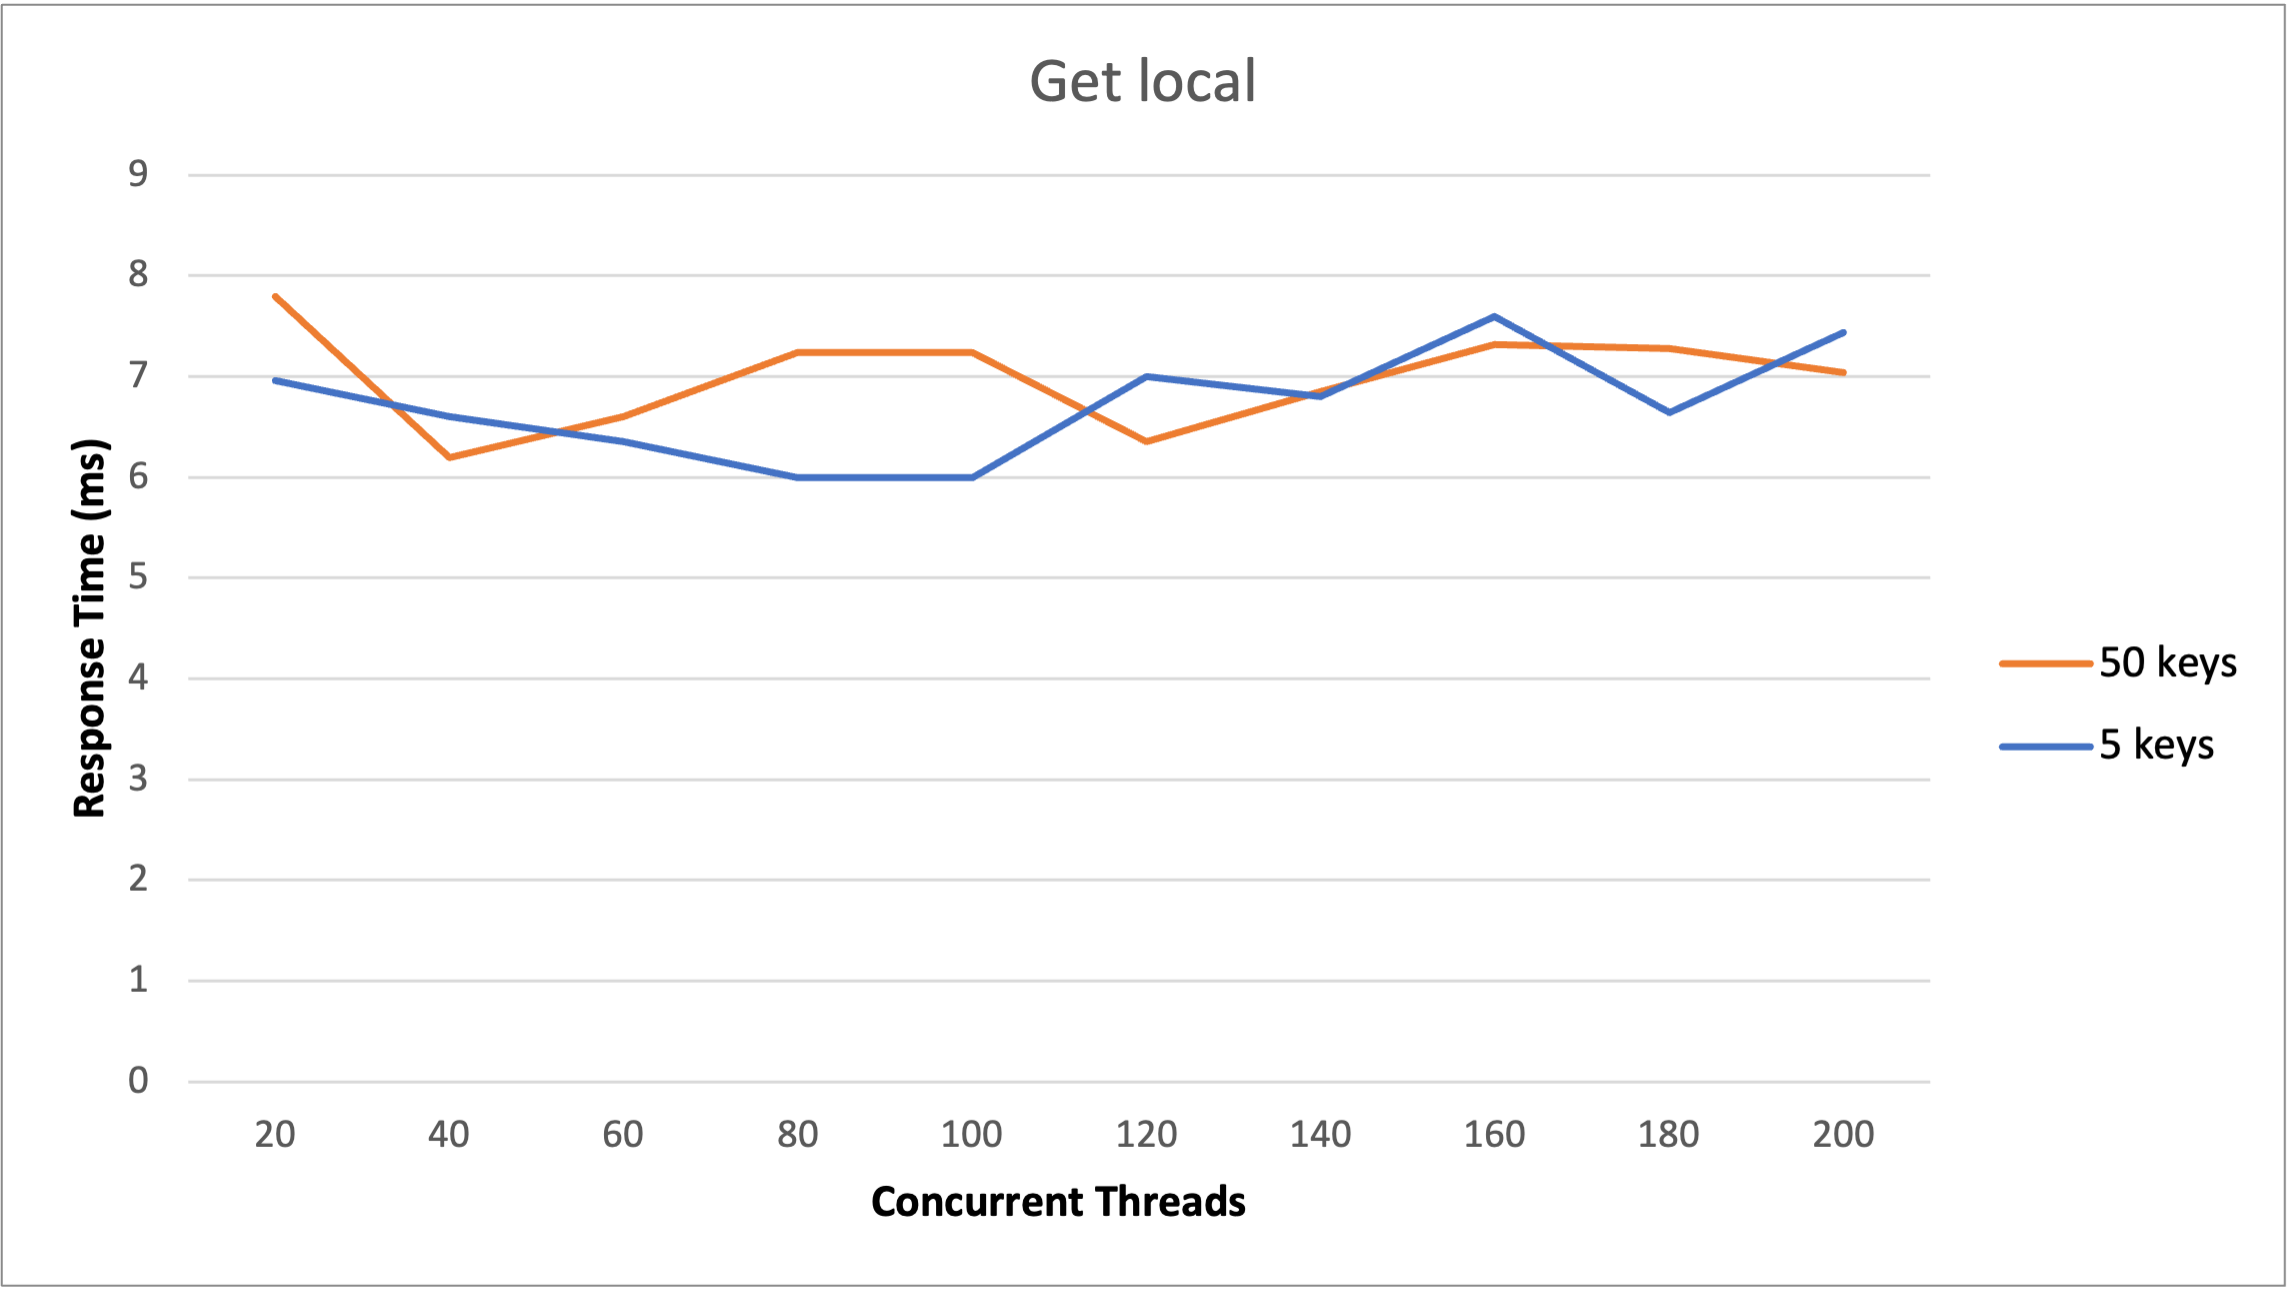
\includegraphics[scale=0.5]{images/getlocal.png}
\end{figure}
\begin{figure}[H]
  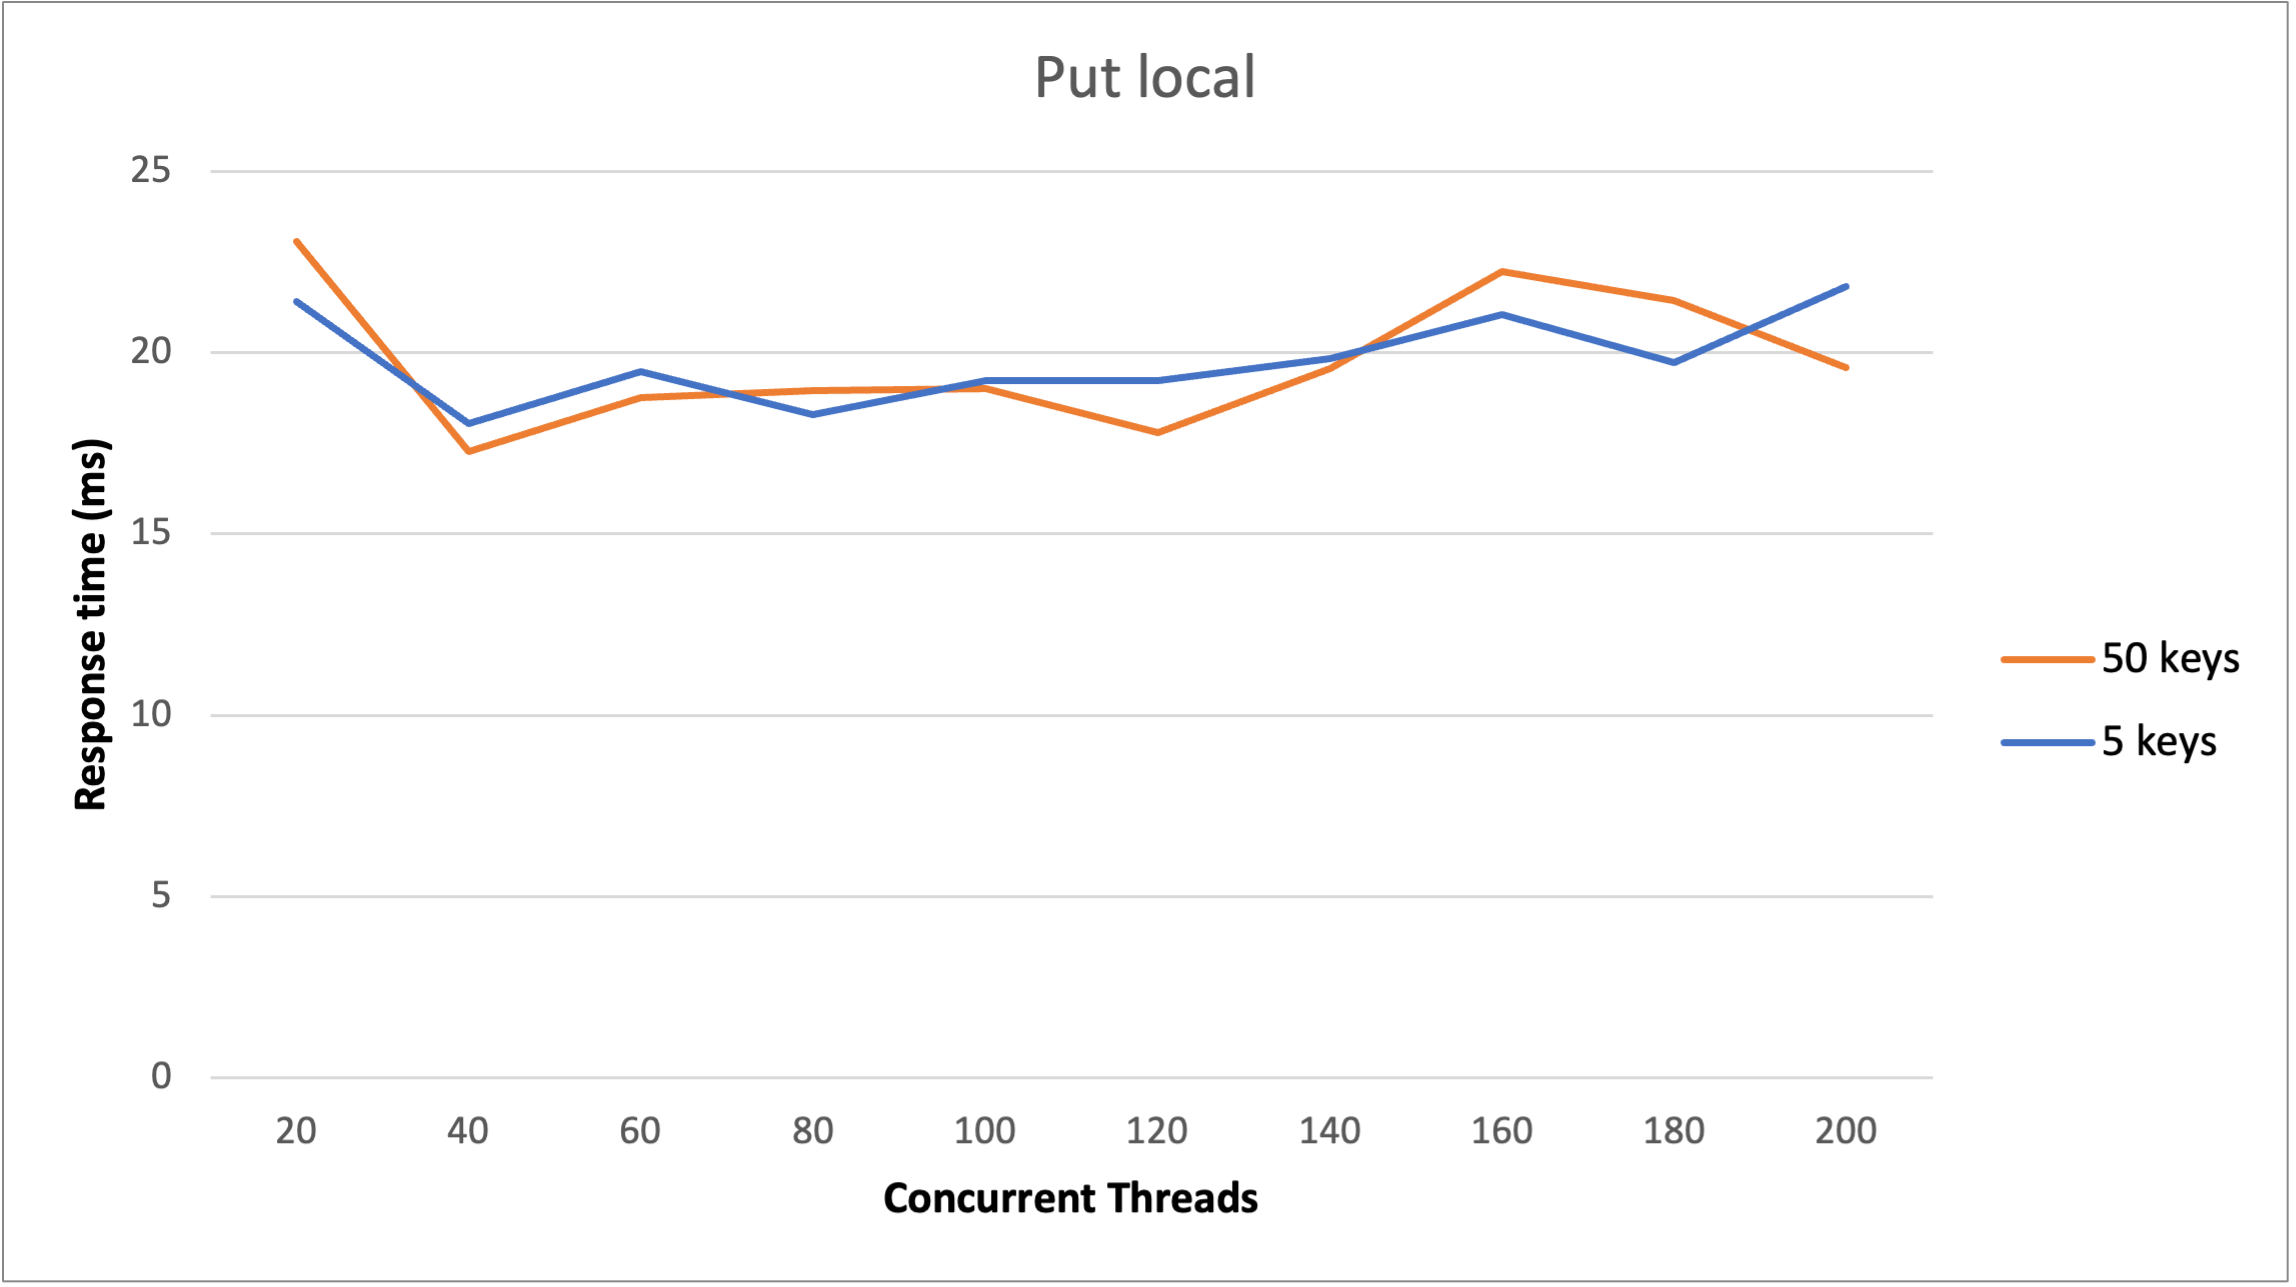
\includegraphics[scale=0.5]{images/putlocal.png}
\end{figure}

\subsubsection{Configurazione 2}
Nel secondo caso di test si può osservare l'influenza del cloud sui tempi di risposta del sistema. Rispetto al caso precedente
si hanno tempi di risposta superiori per le operazioni di get e put.
I thread insistono su un insieme di 5 chiavi.
Con l'aumentare dei thread concorrenti il tempo di risposta delle operazioni di scrittura cresce, mentre il tempo di risposta
delle operazioni di lettura rimane pressoché costante.
\begin{figure}[H]
  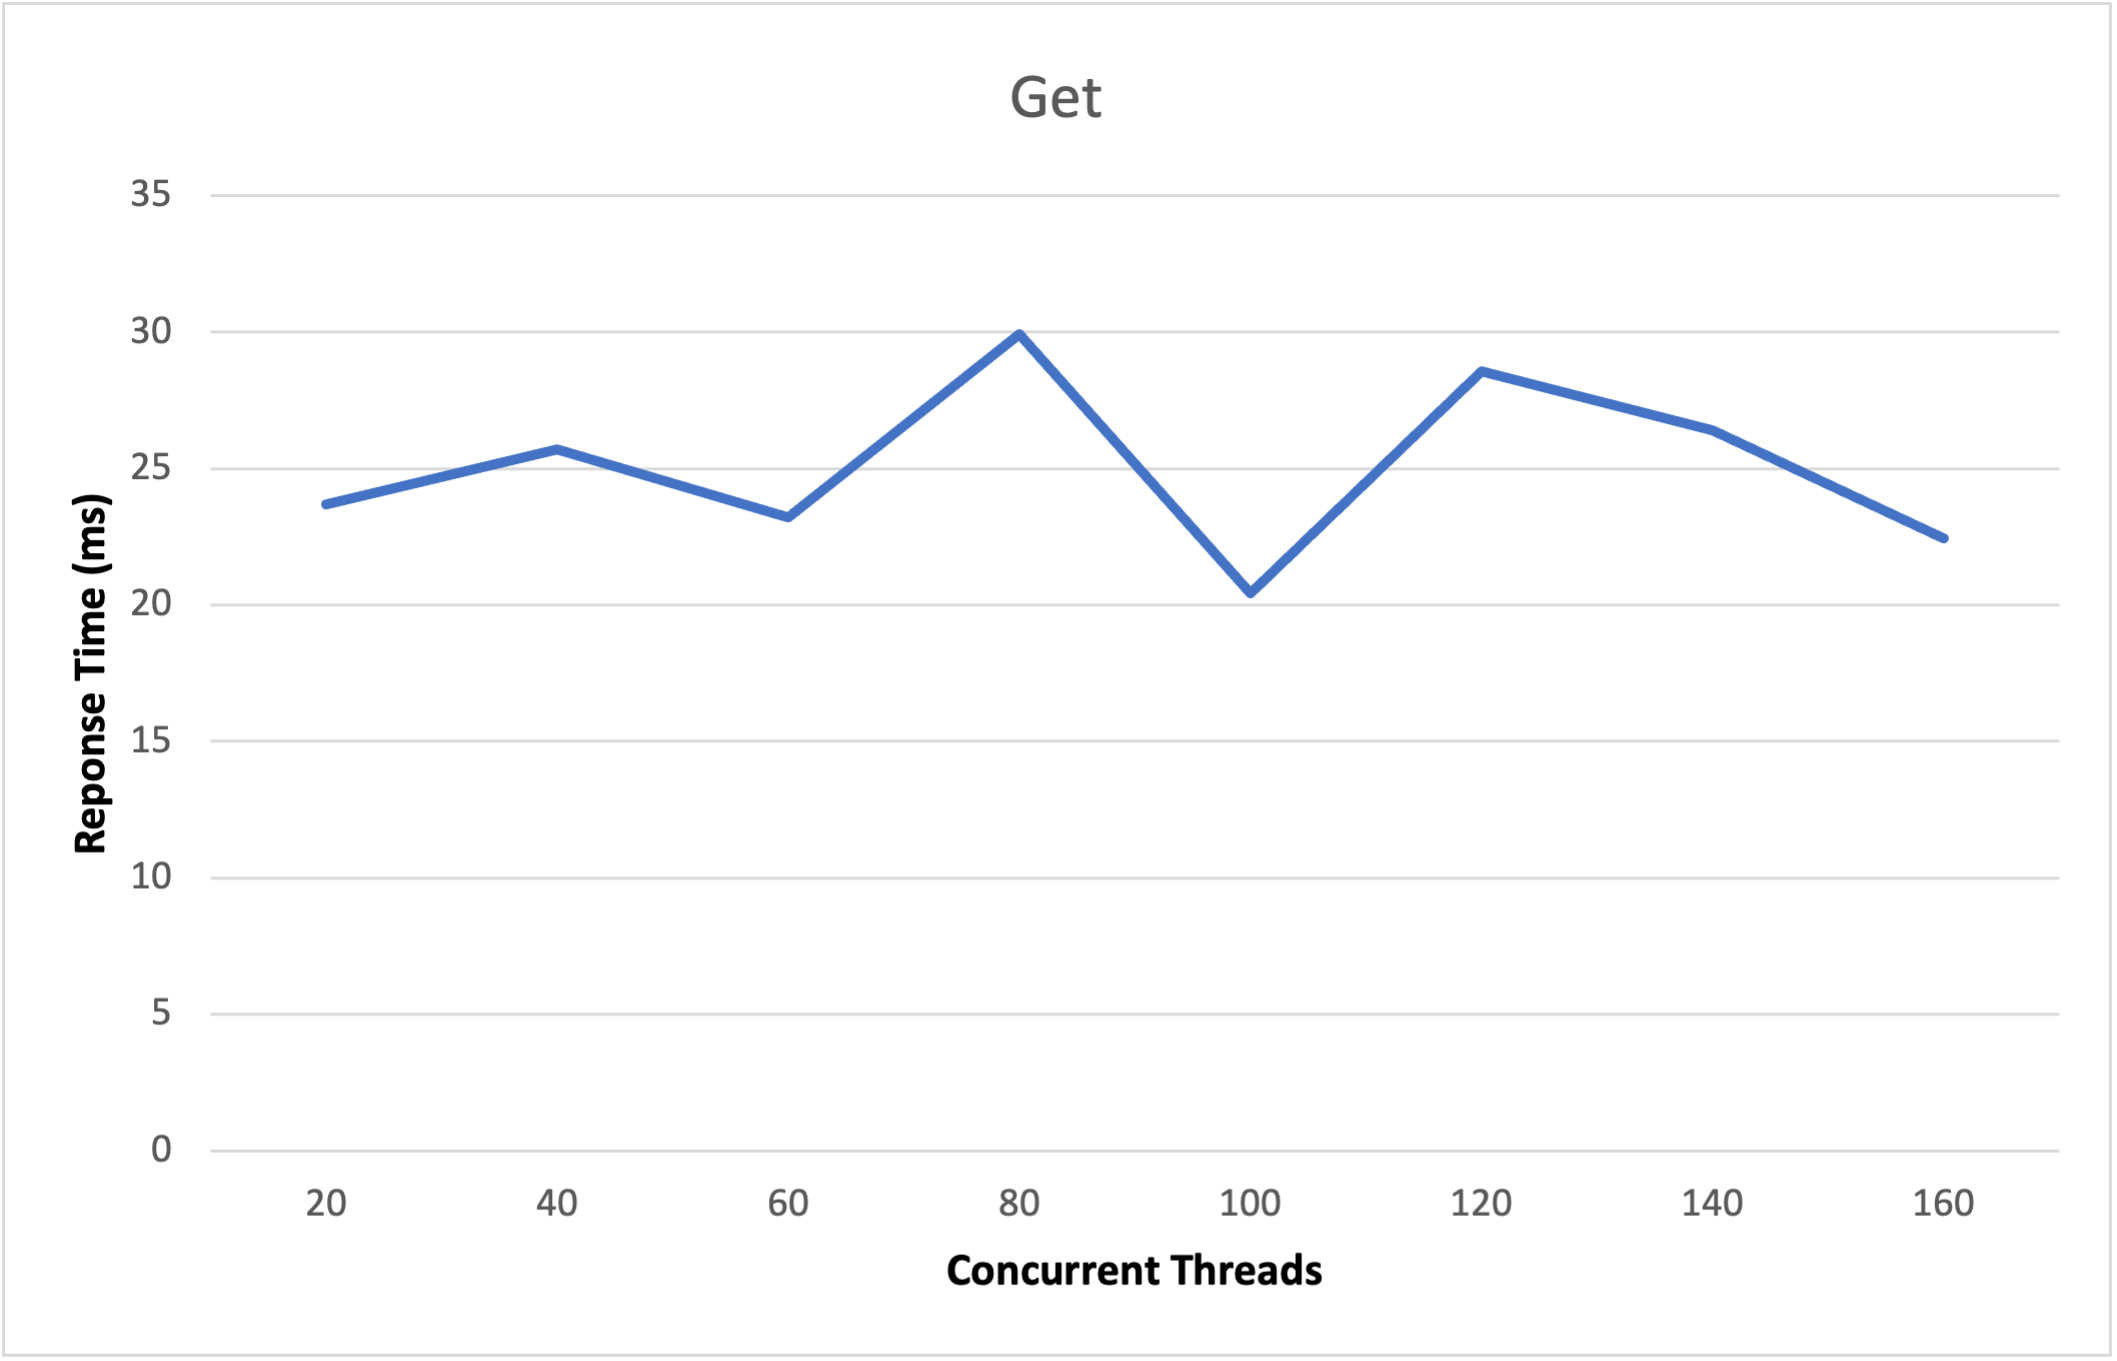
\includegraphics[scale=0.5]{images/get.png}
\end{figure}
\begin{figure}[H]
  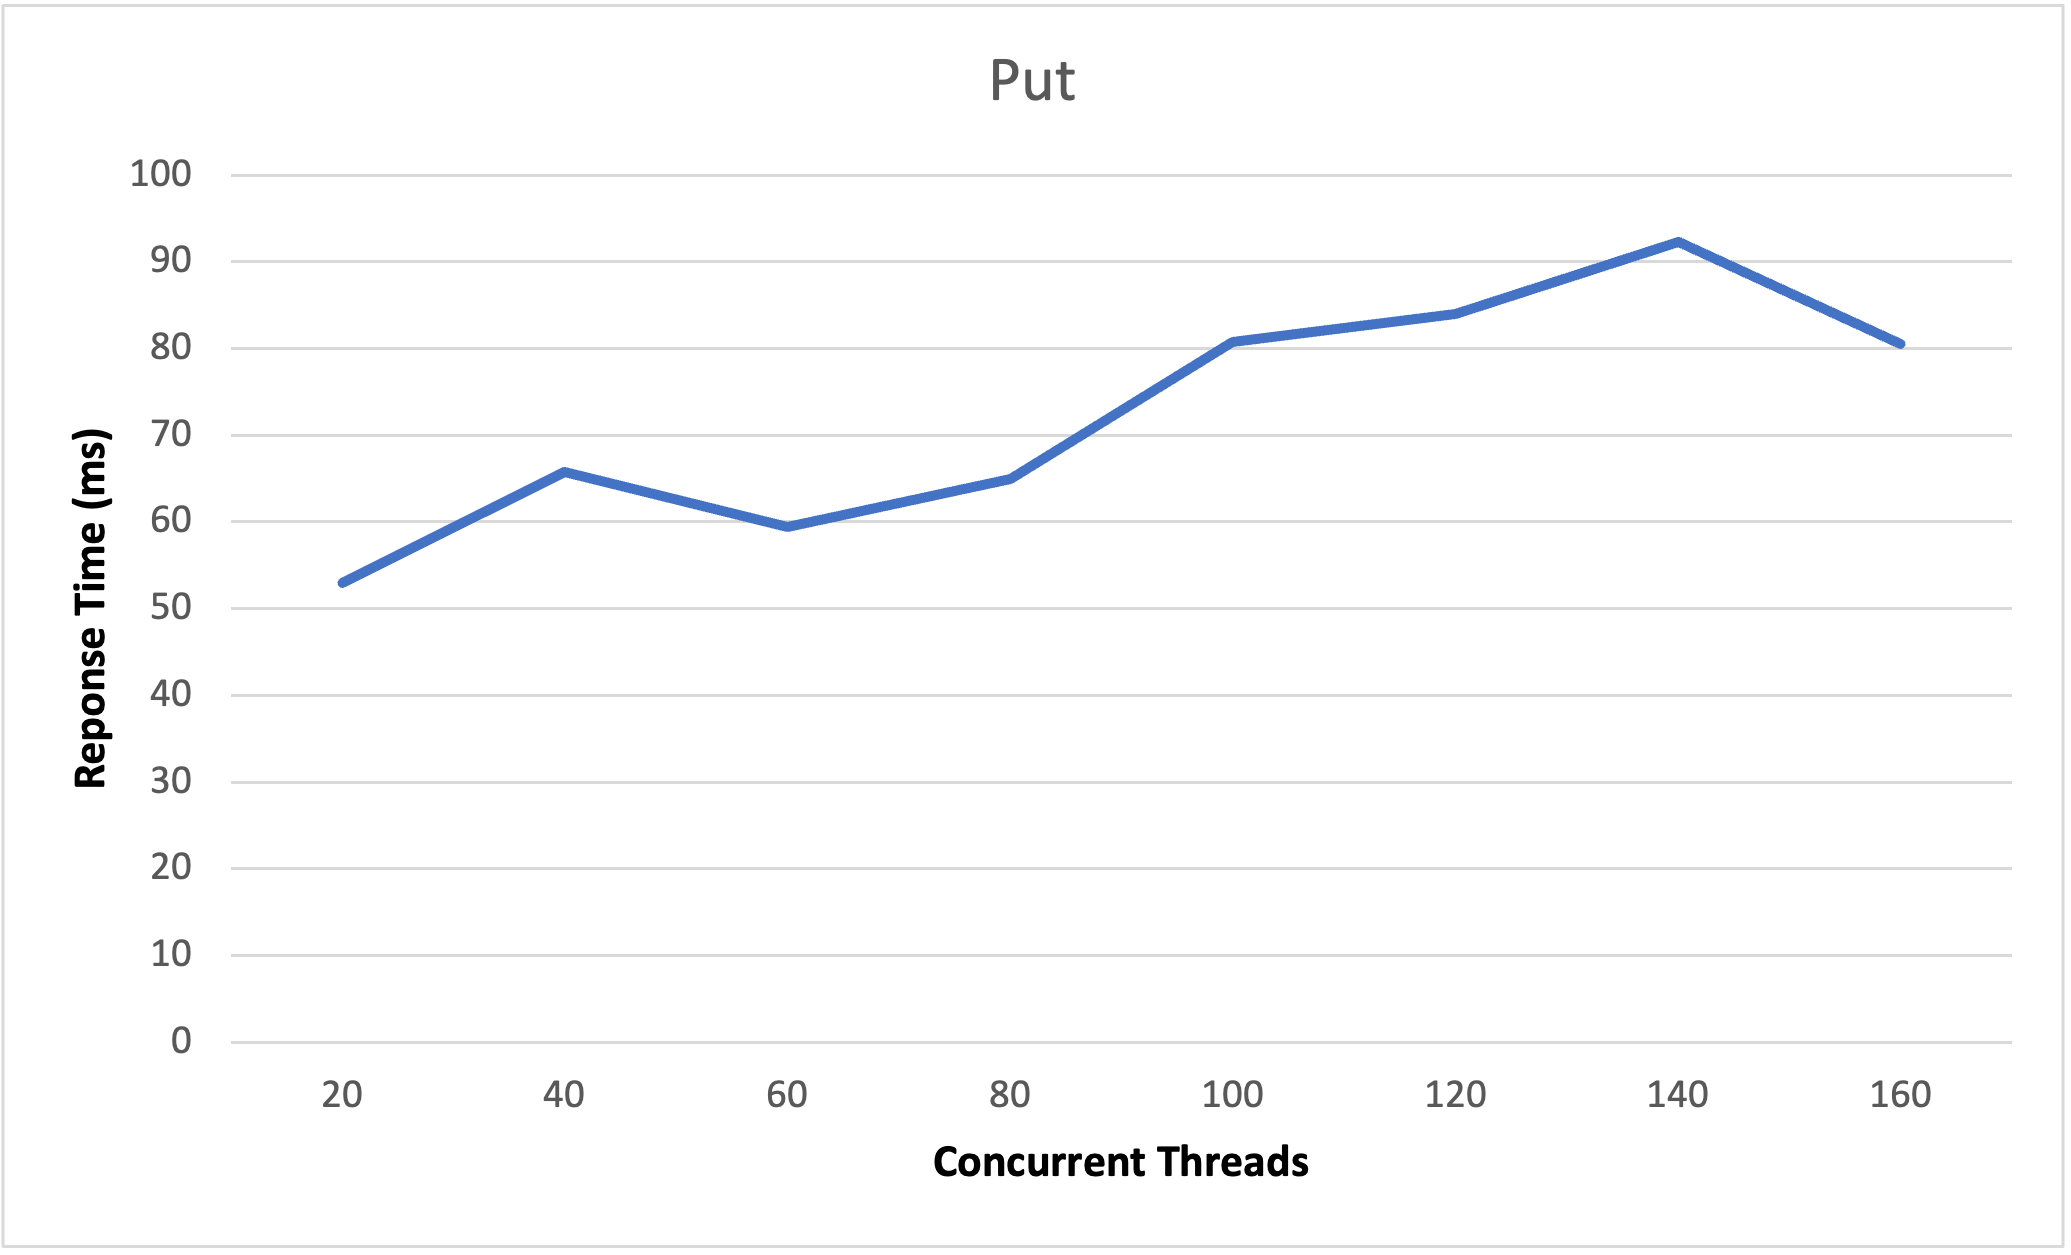
\includegraphics[scale=0.5]{images/put.png}
\end{figure}

\subsubsection{Configurazione 3}
In questo test case si è testato il comportamento del sistema con un numero elevato di thread concorrenti. I dati inseriti
dai vari thread sono compresi tra 1 e 200 byte. Le prestazioni del sistema restano apprezzabili anche con un numero elevato di thread concorrenti.
I thread insistono su un insieme di 100 chiavi.
\begin{figure}[H]
  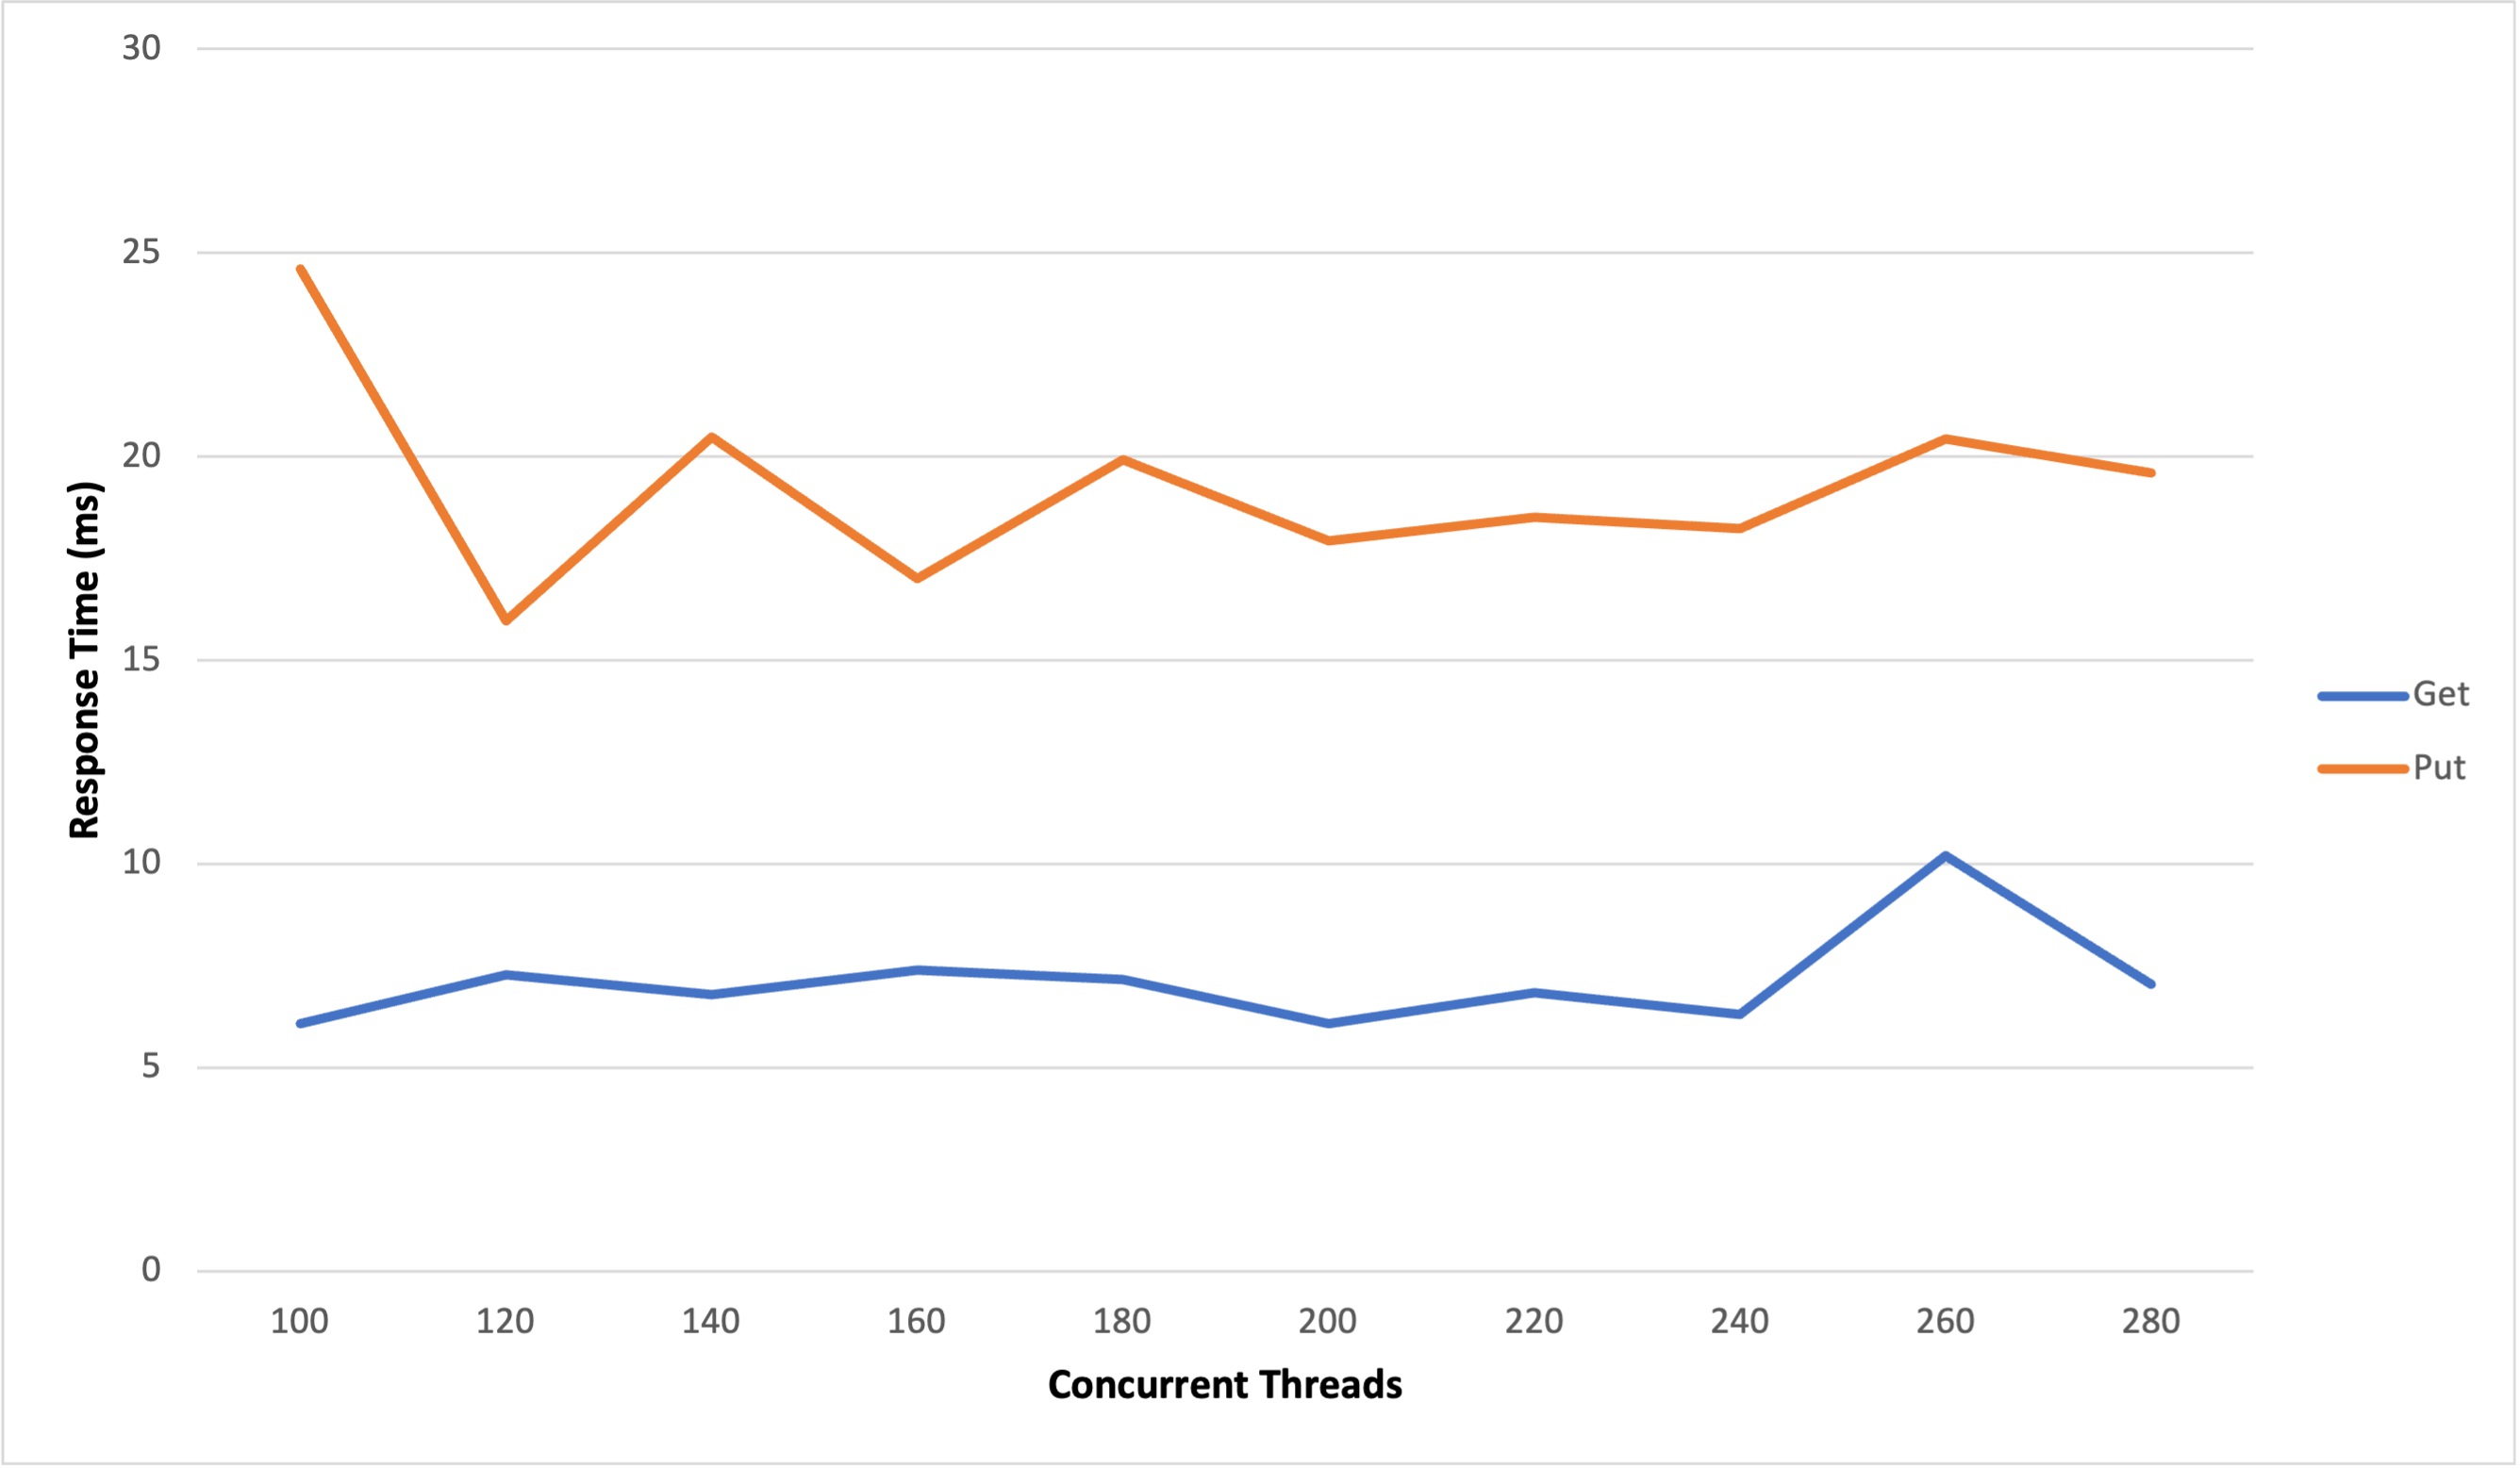
\includegraphics[scale=0.4]{images/stress.png}
\end{figure}

\subsubsection{Configurazione 4}
Da quest'ultimo test case si può osservare il comportamento del sistema con una prevalenza di operazioni di scrittura.
Entrambe le operazioni di scrittura presentano un tempo di risposta simile.
I thread insistono su un insieme di 100 chiavi.
\begin{figure}[H]
  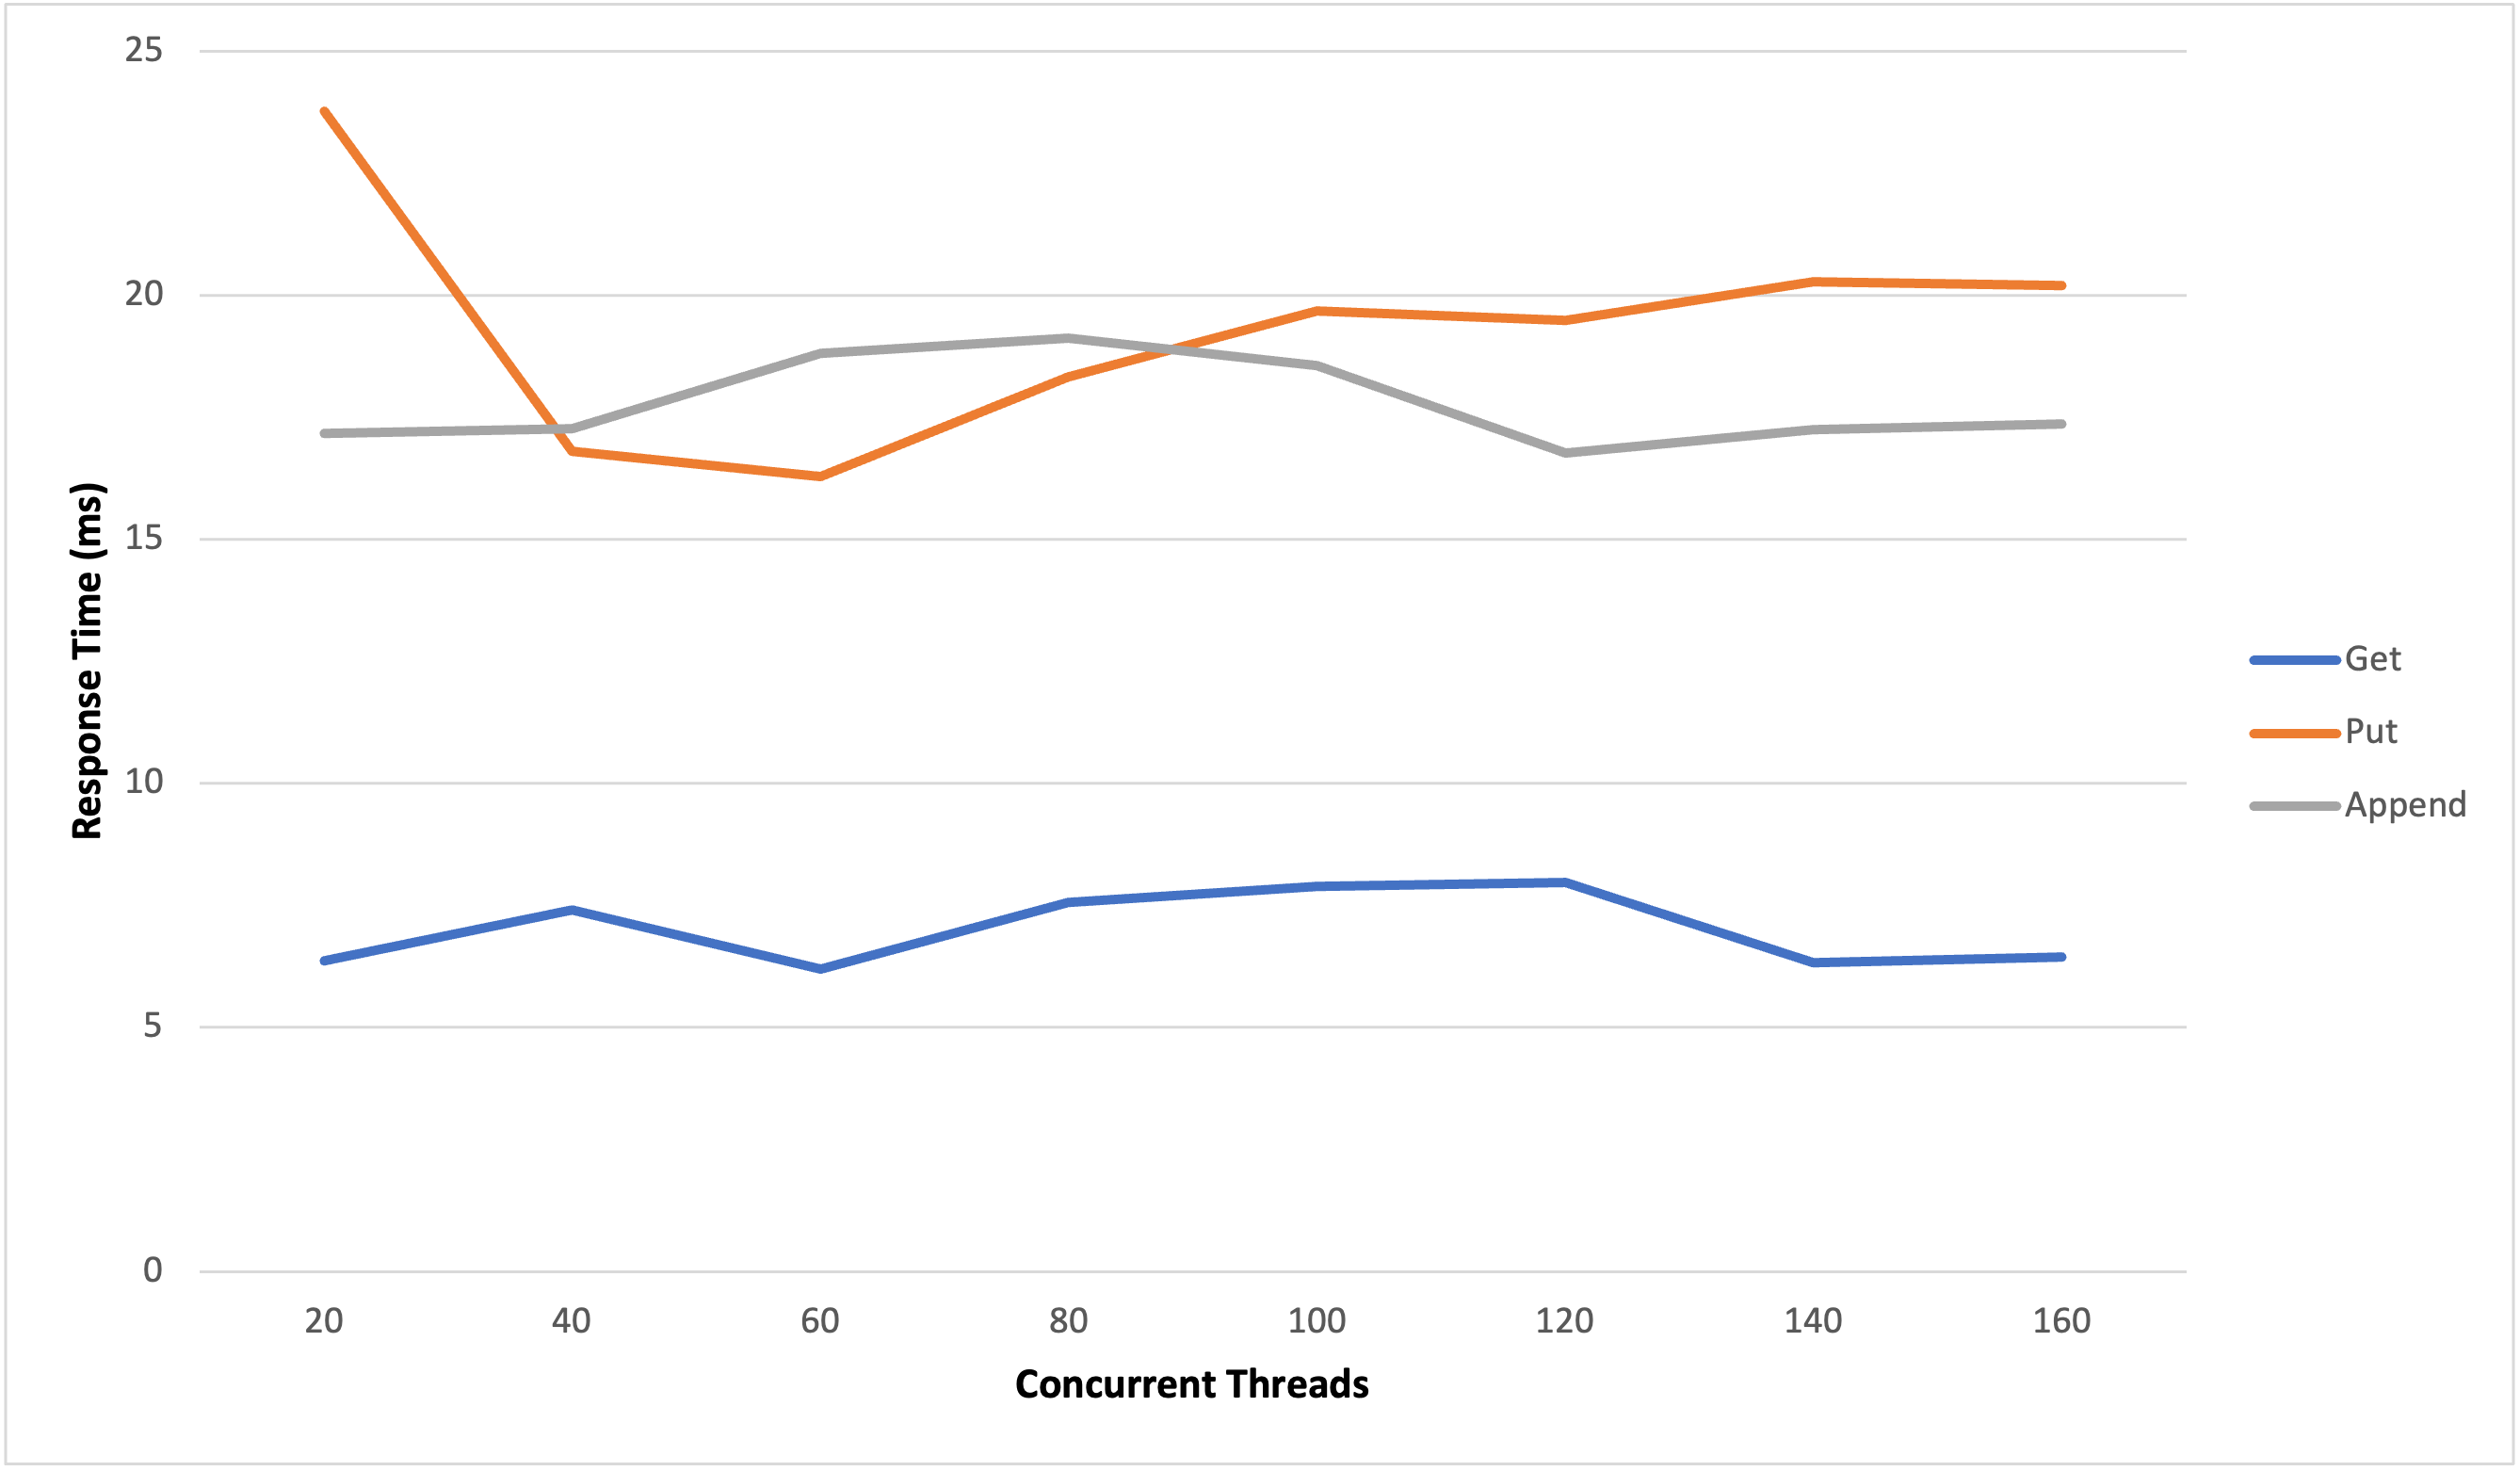
\includegraphics[scale=0.4]{images/conf3.png}
\end{figure}

\section{Manuale d'uso}
Il codice del progetto è reperibile al link \href{https://github.com/ThetaRangers/SDCC}{https://github.com/ThetaRangers/SDCC}.\\
Prima dell'esecuzione, si richiede che sia in esecuzione il servizio di registrazione sul cloud e che le credenziali
AWS siano presenti anche nella cartella .aws della directory principale del progetto. In caso di esecuzione locale, il servizio
di registrazione può essere sostituito con il programma registerServer.go, impostando nel file config.json \verb!"TestingMode": true!.\\
L'applicazione in esecuzione sfrutta la porta 50051 per ricevere
chiamate gRPC, la porta 42424 per interagire con gli altri nodi nelle operazioni correlate alla rete strutturata.

\subsection{Installazione}
Una volta scaricati i file sorgente, è possibile compilarli con il comando \verb!make executable!, che va a generare il
file eseguibile ``server'' C'è anche la possibilità di generare un'immagine docker con il comando \verb!make docker!, che
può essere eseguita con il comando \verb!docker run -it lpn!. Le istruzioni per installare le dipendenze sono presenti nel
file README.md.

\subsection{Configurazione}
Il sistema ha diverse componenti che possono essere configurate senza necessità di ricompilare il codice. Tutte queste
proprietà sono scritte nel file config.json:
\begin{itemize}
  \item {Database} indica il database sfruttato dal singolo nodo come rete locale. Questa proprietà può avere un valore
differente per ogni nodo.
  \item {DbAddress} indica l'indirizzo IP in cui è reperibile il database che implementa lo storage locale del nodo.
Questo indirizzo è particolarmente utile nel caso in cui il database si trovi su un altro container o preveda questa metodologia
di accesso. Non è utilizzato nel caso in cui il database sia Badger.
  \item {RequestTimeoutMilliseconds} indica dopo quanti millisecondi è possibile considerare fallita una chiamata gRPC che non
ha ricevuto alcuna risposta.
  \item {ReplicationFactor} indica la grandezza minima del cluster. Sarebbe buona norma impostare questo valore a \(2k + 1\),
con k il numero massimo di crash tollerabili in contemporanea nello stesso cluster.
  \item {OffloadingThreshold} indica la taglia massima dopo la quale un valore viene mandato sul cloud.
  \item {DynamoTable} indica il nome della tabella DynamoDB usata dai nodi.
  \item {MigrationWindowMinutes} indica dopo quanti minuti si considerano obsolete le operazioni inserite nella struttura dati
adibita alla migrazione.
  \item {MigrationPeriodSeconds} indica dopo quanti secondi un nodo scorre la propria struttura dati per valutare eventuali
richieste di migrazione.
  \item {MigrationThreshold} indica il valore soglia per la somma dei costi delle operazioni riguardanti una singola chiave
al fine di richiedere la migrazione.
  \item {Subnet} indica la maschera di sottorete con la quale un nodo apprende il proprio indirizzo IP. Per forzare un
matching esatto è necessario porre IP/32 come subnet.
  \item {TestingServer} indica l'indirizzo IP del servizio di registrazione locale che esegue il file registerServer.go.
  \item {TestingMode} indica se si sta usando il servizio di registrazione locale o quello implementato su AWS.
  \item {AwsRegion} indica il nome della regione AWS su cui sono presenti i servizi sfruttati dal sistema.
  \item {CostRead} indica il costo delle operazioni di read.
  \item {CostWrite} indica il costo delle operazioni di write.
  \item {MaxKey} indica la taglia massima per la chiave di un dato.
\end{itemize}


\subsection{Esecuzione}
Se è presente un servizio di registrazione, si può eseguire il programma ``server'' compilato su un nodo del sistema, oppure
si può eseguire l'apposito container. I singoli nodi restano in attesa di poter formare un cluster. Nel caso in cui ciò
sia possibile, l'ultimo nodo che ha richiesto la registrazione al servizio notifica i nodi in attesa della formazione di
un cluster tramite apposite chiamate gRPC. Quando il numero di nodi nel sistema è pari o superiore al campo ReplicationFactor
del file config.json, l'insieme dei nodi è in grado di ricevere e gestire connessioni di ingresso da parte dei client.
\subsection{Libreria Client}
I client possono connettersi sfruttando l'apposita libreria, che fornisce un'astrazione per le operazioni di connessione
al sistema e le chiamate a procedura remota. In particolare, è possibile avvalersi di questa per ricevere la lista dei
nodi che compongono il sistema dal servizio di registrazione. Questa lista viene usata dalla libreria per eseguire dei
ping in parallelo, al fine di individuare il nodo che fornisca la latenza minima di rete.
È disponibile anche una command line interface per interagire con il sistema. Per utilizzare la cli si necessita di eseguire
il comando \verb!go run cli.go!. I comandi supportati dalla cli sono:
\begin{itemize}
  \item connect [IP]: per connettersi ad un nodo del sistema
  \item nodes [cloud url]: per ottenere tutti i nodi del sistema
  \item closest [cloud url]: per ottenere il nodo con latenza minore
  \item lnodes [register server addr]: per ottenere tutti i nodi del sistema se si usa il server di testing
  \item lclosest [register server addr]: per ottenere il nodo con latenza minore se si usa il server di testing
  \item put [key] [value...]: per inserire un dato nel sistema
  \item get [key]: per ottenere un dato dal sistema
  \item append [key] [value...]: per eseguire l'operazione di append
  \item del [key]: per cancellare un dato dal sistema
  \item disconnect: per disconnettersi da un nodo
  \item quit: per uscire dalla cli
\end{itemize}
Le sezioni dei comandi indicate tra parentesi quadre sono da intendersi come i parametri di questi. Nel caso in cui
siano presenti anche tre punti, i parametri dello stesso tipo possono essere uno o più, separati da spazi. La cli, attualmente, non supporta
l'inserimento di chiavi o valori contenenti spazi.

\printbibliography

\end{document}
